\chapter{Практическая часть}

Лабораторная работа состоит из двух частей:
\begin{itemize}
    \item[1)] Организовать взаимодействие параллельных процессов на отдельном компьютере.
    \item[2)] Организовать взаимодействие параллельных процессов в сети (ситуацию моделируем на одной машине).
\end{itemize}

\section{Задание \No{}1}
Написать приложение по модели клиент-сервер, демонстрирующее взаимодействие параллельных процессов на отдельном компьютере с использованием сокетов в файловом пространстве имен: семейство - AF\_UNIX, тип - SOCK\_DGRAM.
При демонстрации работы программного комплекса необходимо запустить несколько клиентов (не меньше 5) и продемонстрировать, что сервер обрабатывает обращения каждого запущенного клиента.

\lstset{language=c}
\begin{lstlisting}[caption=Текст программы клиента из первого задания]
#include <stdlib.h>
#include <stdio.h>
#include <string.h>
#include <errno.h>
#include <sys/types.h>
#include <sys/socket.h>
#include <unistd.h>
#include <stdlib.h>

#define SOCK_NAME "socket.soc"
#define BUF_SIZE 256

int main(int argc, char ** argv)
{
    int sock = socket(AF_UNIX, SOCK_DGRAM, 0);
    char buf[BUF_SIZE];
    char msg[BUF_SIZE];
    struct sockaddr srvr_name;

    if (sock < 0)
    {
    perror("socket failed");
    return EXIT_FAILURE;
    }

    srvr_name.sa_family = AF_UNIX;
    strcpy(srvr_name.sa_data, SOCK_NAME);

    printf("message: ");
    scanf("%255s",  msg);

    sprintf(buf, "client %d: %s", getpid(), msg);

    sendto(sock, buf, strlen(buf), 0, &srvr_name,
           strlen(srvr_name.sa_data) + sizeof(srvr_name.sa_family));

    return 0;
}
\end{lstlisting}

В процессе-клиенте создаётся сокет в  файловом пространтве имён (домен AF\_UNIX) с типом SOCK\_DGRAM, что означает, что это датаграммный сокет, затем передаётся сообщение серверу с помощью функции sendto().

\lstset{language=c}
\begin{lstlisting}[caption=Текст программы сервера из первого задания]
#include <stdlib.h>
#include <stdio.h>
#include <string.h>
#include <errno.h>
#include <sys/types.h>
#include <sys/socket.h>
#include <unistd.h>

#define SOCK_NAME "socket.soc"
#define BUF_SIZE 256

int main(int argc, char ** argv)
{
    struct sockaddr srvr_name;
    char buf[BUF_SIZE];
    int sock;
    int namelen, bytes;

    sock = socket(AF_UNIX, SOCK_DGRAM, 0);
    if (sock < 0)
    {
        perror("socket failed");
        return EXIT_FAILURE;
    }
    srvr_name.sa_family = AF_UNIX;
    strcpy(srvr_name.sa_data, SOCK_NAME);
    if (bind(sock, &srvr_name, strlen(srvr_name.sa_data) +
        sizeof(srvr_name.sa_family)) < 0)
    {
        perror("bind failed");
        return EXIT_FAILURE;
    }

    printf("Server is running.\n");
    while (strcmp(buf, "break"))
    {
        bytes = recvfrom(sock, buf, sizeof(buf),  0, NULL, NULL);
        if (bytes < 0)
        {
            perror("recvfrom failed");
            close(sock);
            unlink(SOCK_NAME);
            return EXIT_FAILURE;
        }
        buf[bytes] = 0;
        printf("Client sent: %s\n", buf);
    }

    close(sock);
    unlink(SOCK_NAME);
}
\end{lstlisting}

В процессе-сервере также создаётся датаграммный сокет в файловом пространтсве имён, после чего происходит связка сокета с заданным адресом с помощью функции bind().
Затем в цикле происходит обработка сообщений из клиентов. Для чтения используется функция recvfrom(), блокирующая программу до тех пор, пока на вход не придут новые данные.
Сервер обрабатывает сообщения до тех пор, пока клиент не отправит сообщение "break". После чего сокет закрывается и файл сокета удаляется.

Пример работы сервера, принимающего сообщения от клиентов:
\begin{figure}[H]
    \centering
    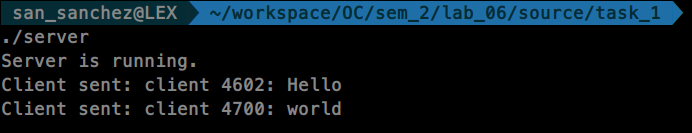
\includegraphics[scale=0.6]{data/image/cor_2.png}
    \caption{Скришот работы сервера.}
\end{figure}
Пример работы клиентов:
\begin{figure}[H]
    \centering
    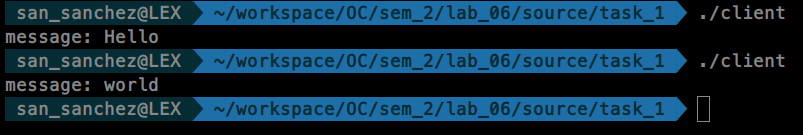
\includegraphics[scale=0.6]{data/image/cor_3.png}
    \caption{Скришот работы клиента.}
\end{figure}

Примеры, показывающие сокет в файловой системе (socket.soc):
\begin{figure}[H]
    \centering
    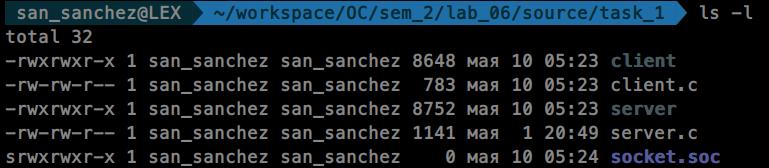
\includegraphics[scale=0.38]{data/image/cor_1.png}
    \caption{Скришот комманды ls -l.}
\end{figure}


\section{Задание \No{}2}

Написать приложение по модели клиент-сервер, осуществляющее взаимодействие параллельных процессов, которые выполняются на разных компьютерах. Для взаимодействия с клиентами сервер должен использовать мультиплексирование. Сервер должен обслуживать запросы параллельно запущенных клиентов. При демонстрации работы программного комплекса необходимо запустить несколько клиентов (не меньше 5) и продемонстрировать, что сервер обрабатывает обращения каждого запущенного клиента.

\lstset{language=c}
\begin{lstlisting}[caption=Текст программы клиента]
#include <stdio.h>
#include <stdlib.h>
#include <errno.h>
#include <string.h>
#include <sys/types.h>
#include <sys/socket.h>
#include <netinet/in.h>
#include <netdb.h>
#include <unistd.h>

#define BUF_SIZE 256

int main(int argc, char ** argv)
{
    int sock, port;
    int pid;
    struct sockaddr_in serv_addr;
    struct hostent *server;
    char buf[BUF_SIZE];
    char buf_answer[BUF_SIZE];

    if (argc < 3)
    {
        fprintf(stderr,"usage: %s <hostname> <port_number>\n", argv[0]);
        return EXIT_FAILURE;
    }

    pid = getpid();

    sock = socket(AF_INET, SOCK_STREAM, 0);
    if (sock < 0)
    {
        printf("socket() failed: %d", errno);
        return EXIT_FAILURE;
    }

    server = gethostbyname(argv[1]);
    if (server == NULL)
    {
        printf("Host not found\n");
        return EXIT_FAILURE;
    }

    serv_addr.sin_family = AF_INET;
    memcpy((char *)&serv_addr.sin_addr.s_addr, (char *)server->h_addr,
            server->h_length);
    port = atoi(argv[2]);
    serv_addr.sin_port = htons(port);

    if (connect(sock, (struct sockaddr*) &serv_addr,
                sizeof(serv_addr)) < 0)
    {
        printf("connect() failed: %d", errno);
        return EXIT_FAILURE;
    }

    sprintf(buf, "%d", pid);
    write(sock, buf, BUF_SIZE);

    printf("Client %d:\n", pid);

    while (strcmp(buf, "break\n"))
    {
        memset(buf, 0, BUF_SIZE);
        printf("Message: ");
        fgets(buf, BUF_SIZE-1, stdin);
        write(sock, buf, strlen(buf));

        memset(buf_answer, 0, BUF_SIZE);
        read(sock, buf_answer, BUF_SIZE-1);
        printf("Answer: %s\n",buf_answer);
    }

    close(sock);
    return 0;
}
\end{lstlisting}

В процессе-клиенте создаётся сокет семейства AF\_INET с типом SOCK\_STREAM. С помощью функции gethostbyname() доменный адрес преобразуется в сетевой, после чего устанавливается соединение с помощью connect(). Затем используются read()/write() для чтения-записи из сокета. Клиент продолжает работу до тех пор, пока не будет послано сообщение break, после чего сокет закрывается.

\lstset{language=c}
\begin{lstlisting}[caption=Текст программы сервера]
#include <stdio.h>
#include <stdlib.h>
#include <errno.h>
#include <string.h>
#include <sys/types.h>
#include <sys/socket.h>
#include <netinet/in.h>
#include <unistd.h>

#define BUF_SIZE 256
#define MAX_CONNECT 1024
#define ANSWER "OK"
#define SIZE_ANSWER 2

typedef struct client client_t;
struct client {
    int fd;
    int pid;
};

int new_connection(int sock, client_t clients[FD_SETSIZE], fd_set *all_set,
        fd_set *reset, int *max_fd, int *max_idx);
int clients_handler(client_t clients[FD_SETSIZE], fd_set *all_set,
        fd_set *reset, int *max_idx);

int main(int argc, char ** argv)
{
    int sock, newsock, port;
    client_t clients[FD_SETSIZE];
    int max_fd, max_idx;
    struct sockaddr_in serv_addr, cli_addr;
    if (argc < 2)
    {
        fprintf(stderr,"usage: %s <port_number>\n", argv[0]);
        return EXIT_FAILURE;
    }

    sock = socket(AF_INET, SOCK_STREAM, 0);
    if (socket < 0)
    {
        printf("socket() failed: %d\n", errno);
        return EXIT_FAILURE;
    }

    memset((char *) &serv_addr, 0, sizeof(serv_addr));
    serv_addr.sin_family = AF_INET;
    serv_addr.sin_addr.s_addr = INADDR_ANY;
    port = atoi(argv[1]);
    serv_addr.sin_port = htons(port);

    if (bind(sock, (struct sockaddr *) &serv_addr,
                sizeof(serv_addr)) < 0)
    {
        printf("bind() failed: %d\n", errno);
        return EXIT_FAILURE;
    }

    printf("Server is running.\n");

    listen(sock, MAX_CONNECT);

    max_fd = sock;
    max_idx = -1;

    fd_set reset, all_set;
    FD_ZERO(&all_set);
    FD_SET(sock, &all_set);

    for (int i = 0; i < FD_SETSIZE; i++)
    {
        clients[i].fd = -1;
    }

    while (1)
    {
        reset = all_set;

        select(max_fd + 1, &reset, NULL, NULL, NULL);

        if (new_connection(sock, clients, &all_set, &reset, &max_fd,
                    &max_idx) != 0)
        {
            return EXIT_FAILURE;
        }
        if (clients_handler(clients, &all_set, &reset, &max_idx) != 0)
        {
            return EXIT_FAILURE;
        }
    }

    close(sock);
}

int new_connection(int sock, client_t clients[FD_SETSIZE], fd_set *all_set,
        fd_set *reset, int *max_fd, int *max_idx)
{
    if (FD_ISSET(sock, reset))
    {
        int conn_fd = accept(sock, NULL, NULL);
        if (conn_fd < 0)
        {
            printf("accept() failed: %d\n", errno);
            return EXIT_FAILURE;
        }

        int idx;
        for (idx = 0; idx < FD_SETSIZE; idx++)
        {
            if (clients[idx].fd < 0)
            {
                clients[idx].fd = conn_fd;
                break;
            }
        }
        if (idx == FD_SETSIZE)
        {
            perror("Maximum number of clients reached\n");
            return EXIT_FAILURE;
        }
        if (idx > *max_idx)
        {
            *max_idx = idx;
        }
        if (conn_fd > *max_fd)
        {
            *max_fd = conn_fd;
        }

        char pid[BUF_SIZE];
        read(conn_fd, pid, BUF_SIZE);
        clients[idx].pid = atoi(pid);

        FD_SET(conn_fd, all_set);
        printf("New client: %d\n", clients[idx].pid);
    }

    return 0;
}

int clients_handler(client_t clients[FD_SETSIZE], fd_set *all_set,
        fd_set *reset, int *max_idx)
{
    char buf[BUF_SIZE];
    int msg_size = 0;
    for (int i = 0; i <= *max_idx; i++)
    {
        if (clients[i].fd == -1)
        {
            continue;
        }

        if (FD_ISSET(clients[i].fd, reset))
        {
            msg_size = read(clients[i].fd, buf, BUF_SIZE);
            if (msg_size == 0)
            {
                close(clients[i].fd);
                FD_CLR(clients[i].fd, all_set);
                clients[i].fd = -1;
                printf("Client %d disconnected\n", clients[i].pid);
            }
            else
            {
                write(clients[i].fd, ANSWER, SIZE_ANSWER);
                buf[msg_size] = '\0';
                printf("Message from %d client: %s", clients[i].pid, buf);
            }
        }
    }

    return 0;
}
\end{lstlisting}

В процессе-сервере также создаётся сокет семейства AF\_INET с типом SOCK\_STREAM. Затем происходит связывание сокета с заданным адресом.
Далее ожидаются запросы на соединение с помощью listen().
После чего инициализируются вспомогательные значения для работы сервера и устанавливаеется новое значение в набор дескрипторов с помощью функции FD\_SET.

Затем сервер блокируется на функции select() до тех пор, пока не будет установлено новое клиентское соединение или на существующее не придут новые данные.
После выхода из блокировки происходит обработка соответсвующих событий.

В функции new\_connection() происходит соединение в ответ на запрос клиента с помощью функции accept(), которая возвращает новый сокет для связи с клиентом. Также мы добавляем новый дескриптор файла (сокет) в набор дескрипторов.

В функции clients\_handler() происходит проверка клиентов на наличие данных, после чего происходит чтение сообщения и ответ клиенту, либо закрытие сокета close() и удаление из набора дескрипторов FD\_CLR(), если клиент отключился.

В примерах работы приложения используется 9898 порт:

\begin{figure}[H]
    \centering
    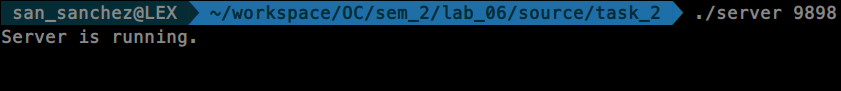
\includegraphics[scale=0.4]{data/image/cor_4.png}
    \caption{Скришот запущенного сервера.}
\end{figure}
\begin{figure}[H]
    \centering
    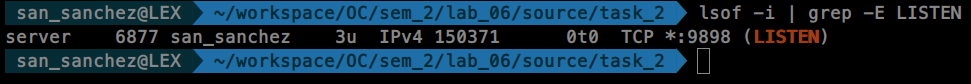
\includegraphics[scale=0.4]{data/image/cor_5.png}
    \caption{Скришот работы команды lsof -i | grep -E LISTEN.}
\end{figure}


Примеры работы второго задания:
\begin{figure}[H]
    \centering
    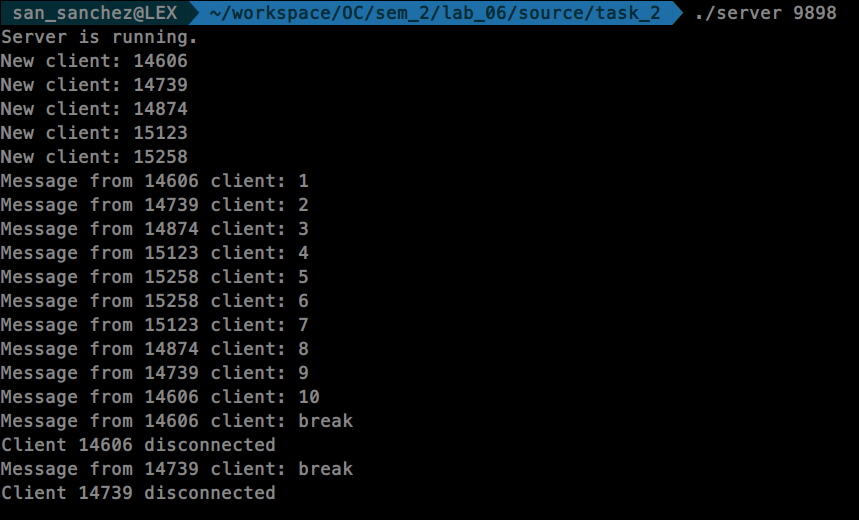
\includegraphics[scale=0.4]{data/image/server_1.png}
    \caption{Скришот работы сервера.}
\end{figure}

\begin{figure}[H]
    \centering
    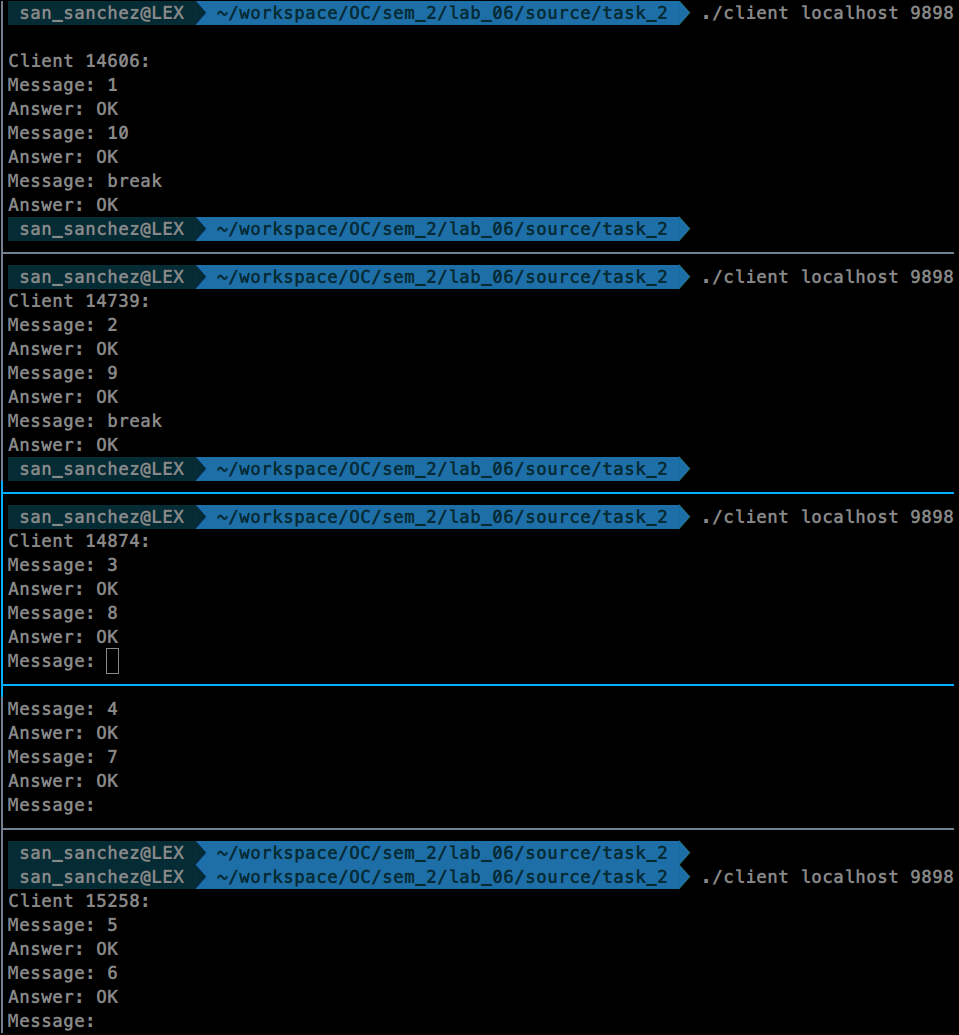
\includegraphics[scale=0.4]{data/image/clietns_1.png}
    \caption{Скришот работы клиентов.}
\end{figure}

\begin{figure}[H]
    \centering
    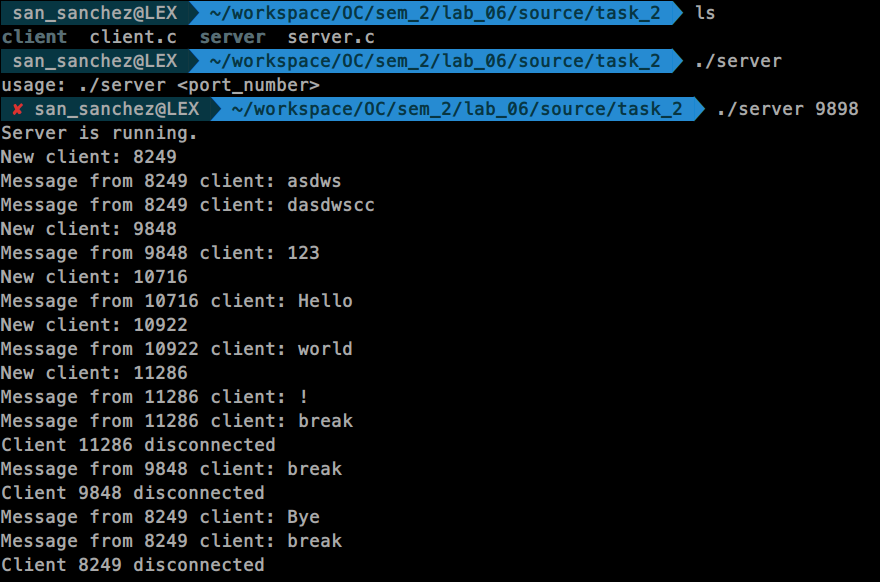
\includegraphics[scale=0.4]{data/image/server_2.png}
    \caption{Скришот работы сервера.}
\end{figure}

\begin{figure}[H]
    \centering
    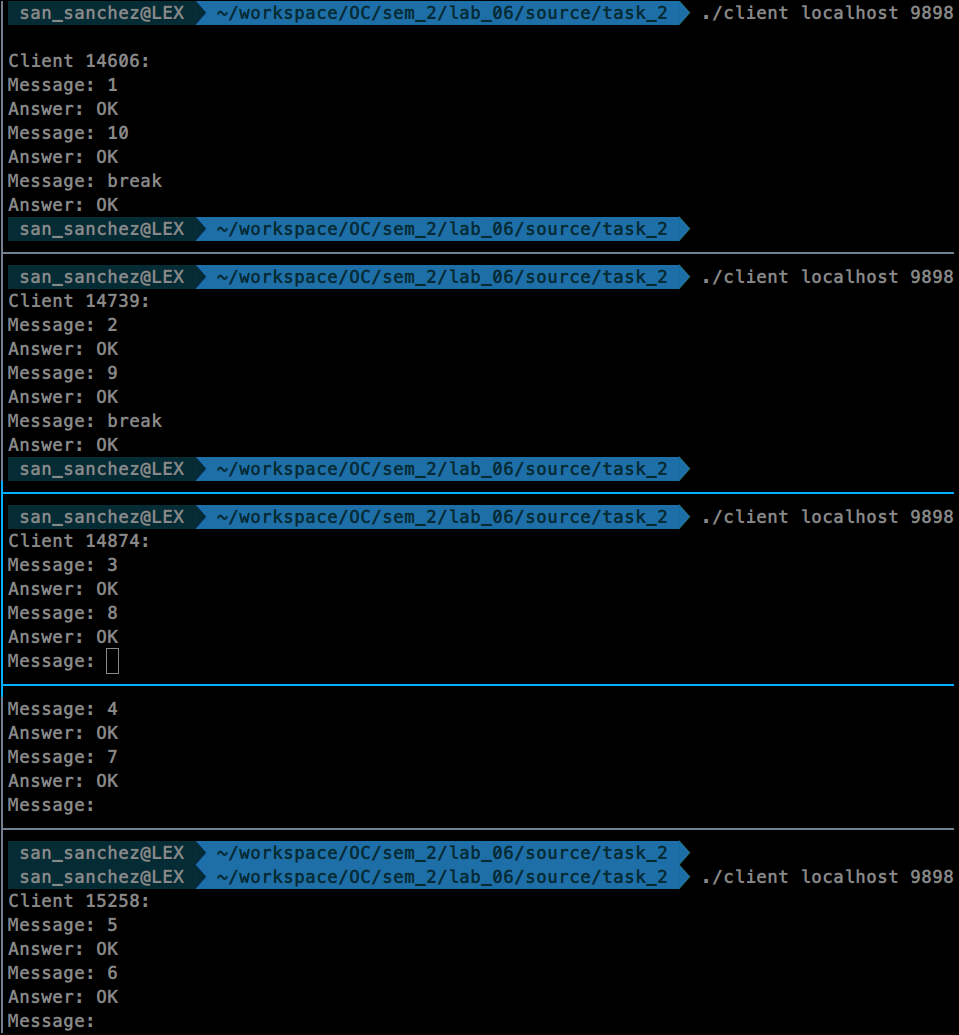
\includegraphics[scale=0.4]{data/image/clietns_1.png}
    \caption{Скришот работы клиентов.}
\end{figure}
